\section{The German Electricity Market}

\subsection{Installed capacities}

\begin{frame}{Installed capacities}
					
\begin{figure}[h]
  \centering
%\caption{Installed capacities in GW of major players in Germany}
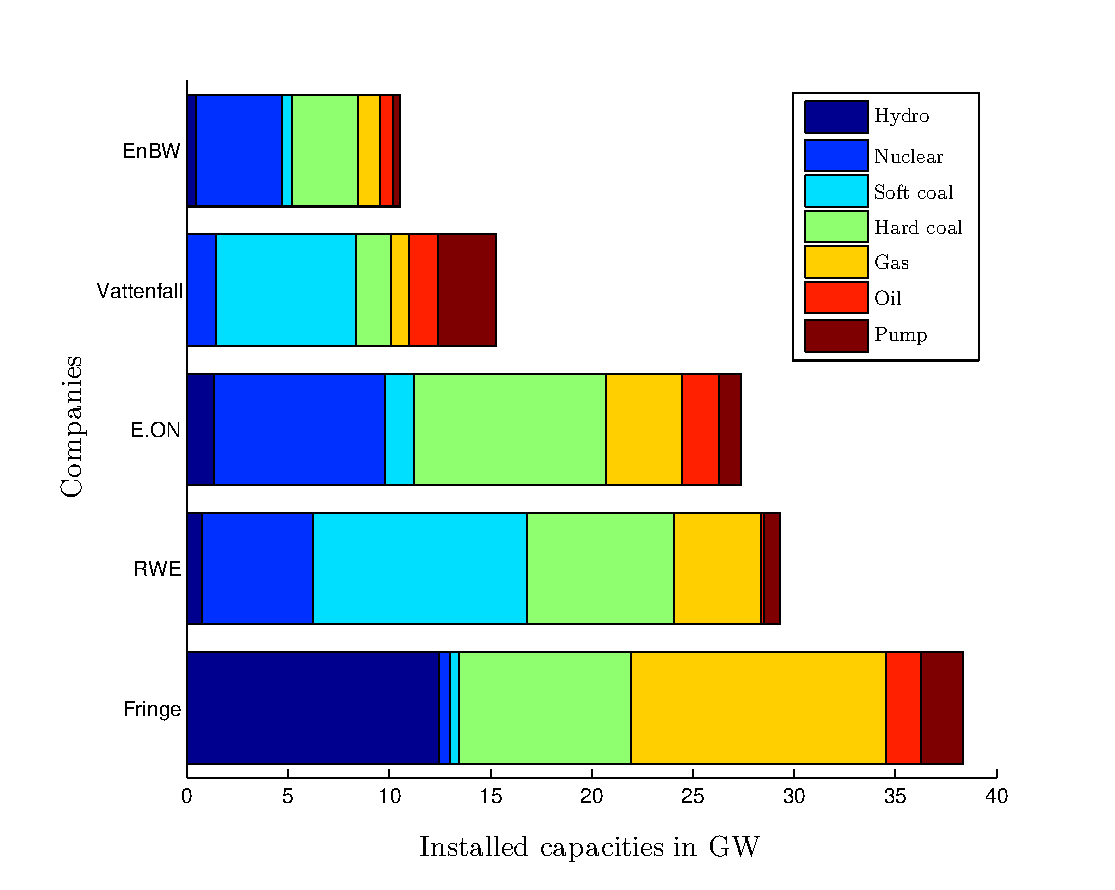
\includegraphics[width=0.85\textwidth]{capacities}
  \label{fig:capacities}
\end{figure}

\end{frame}

\subsection{Electricity load and prices}

\begin{frame} {Electricity load}
					
\begin{figure}[h]
\centering
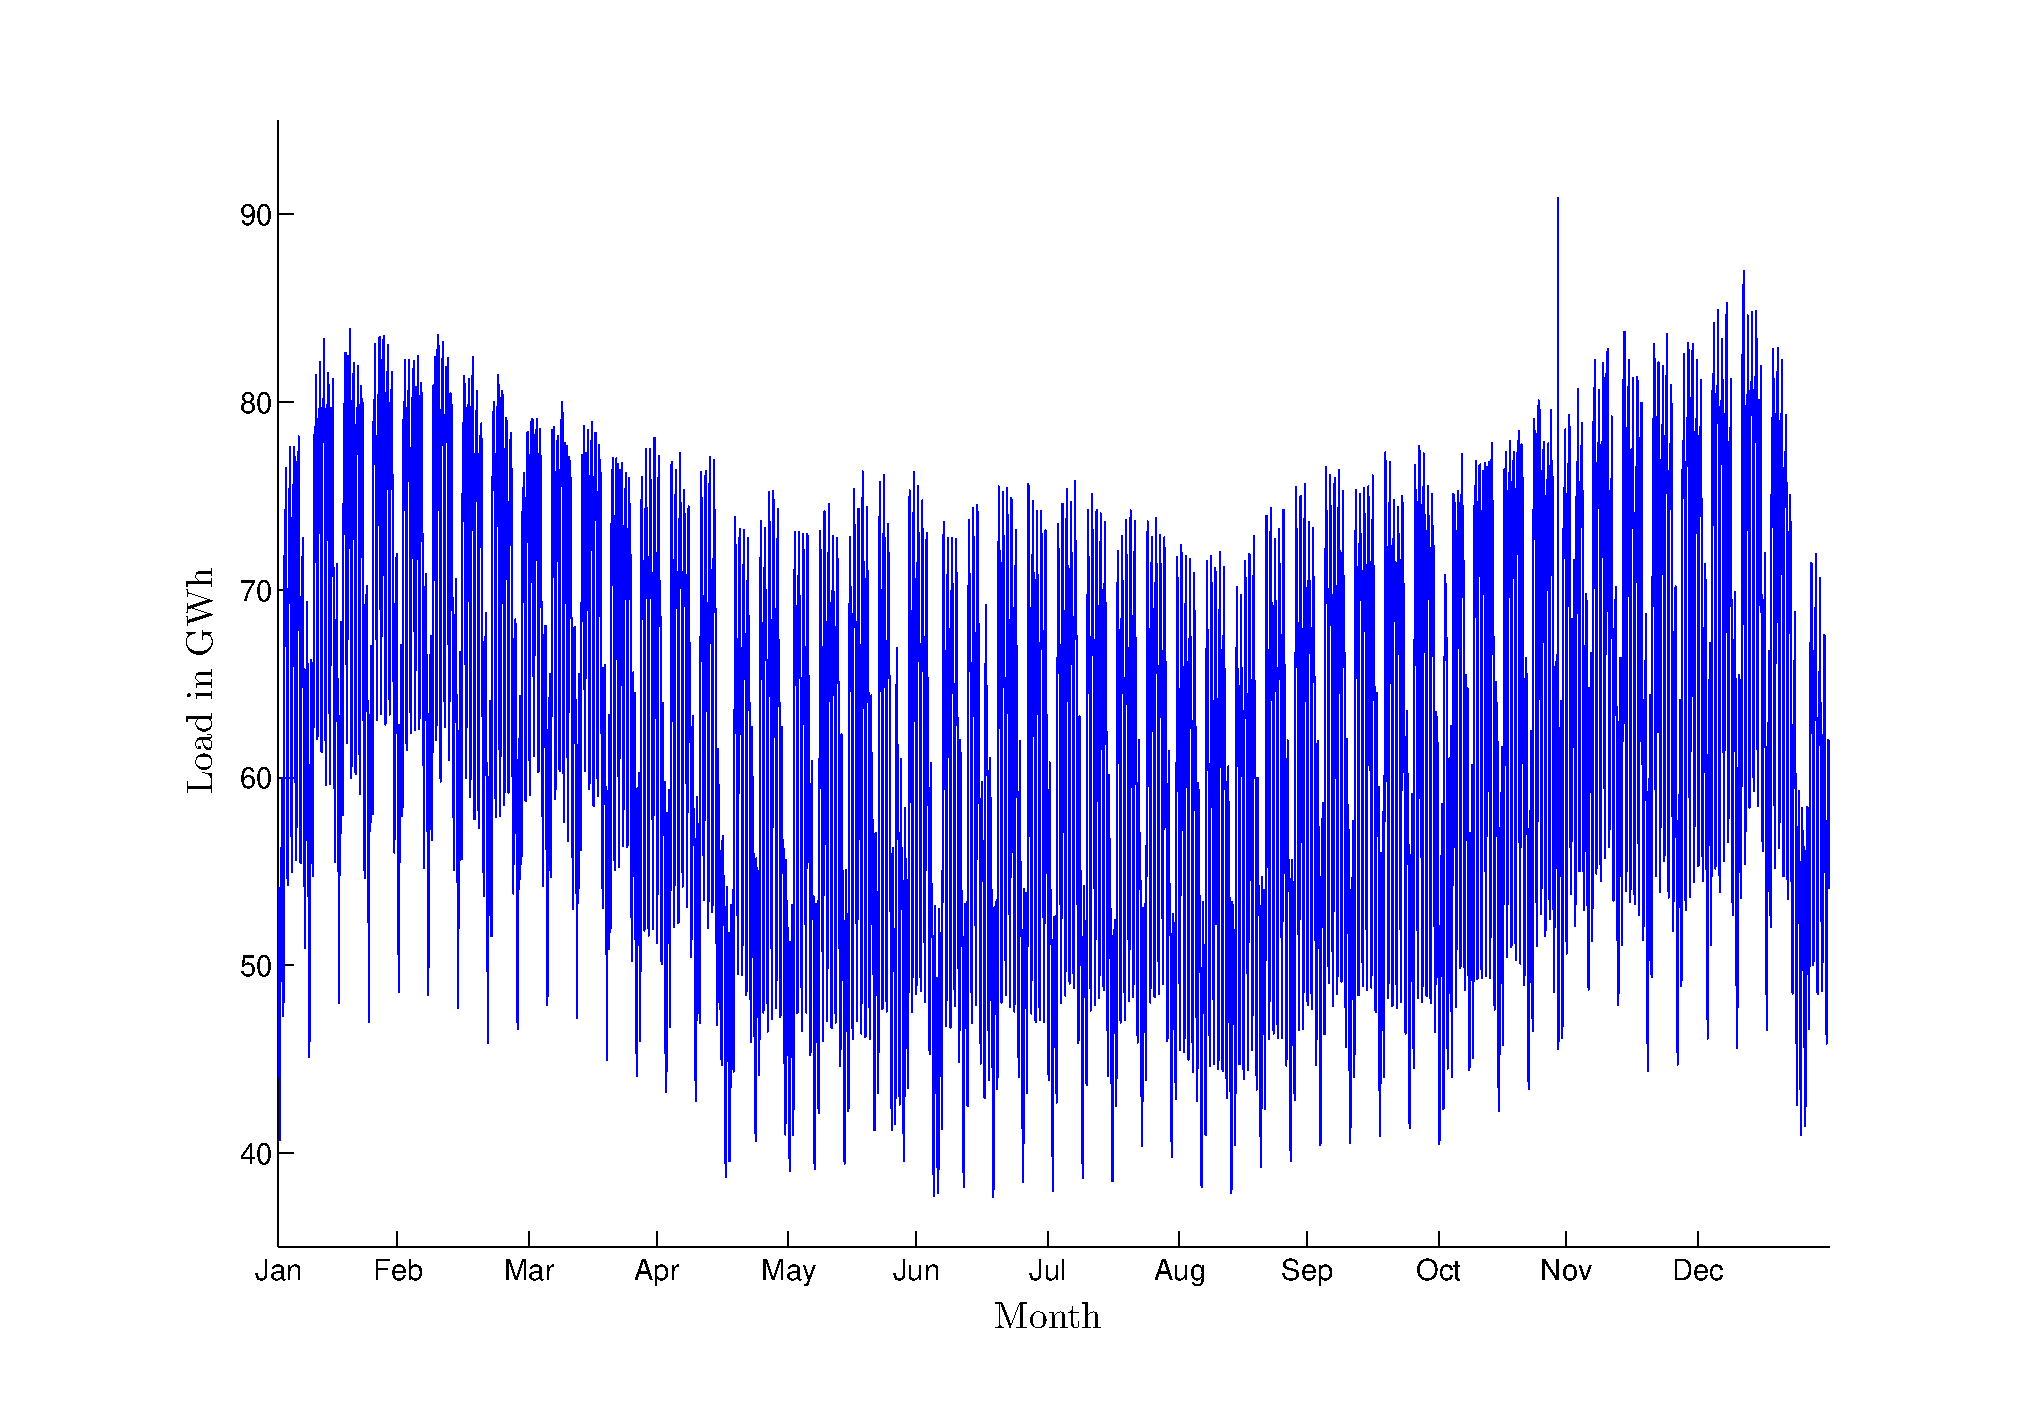
\includegraphics[width=1.0\textwidth, angle=0]{loadvalues}
    \label{fig:load}            
\end{figure}
\end{frame}

\begin{frame} {Electricity prices}				
\begin{figure}[h]
\centering
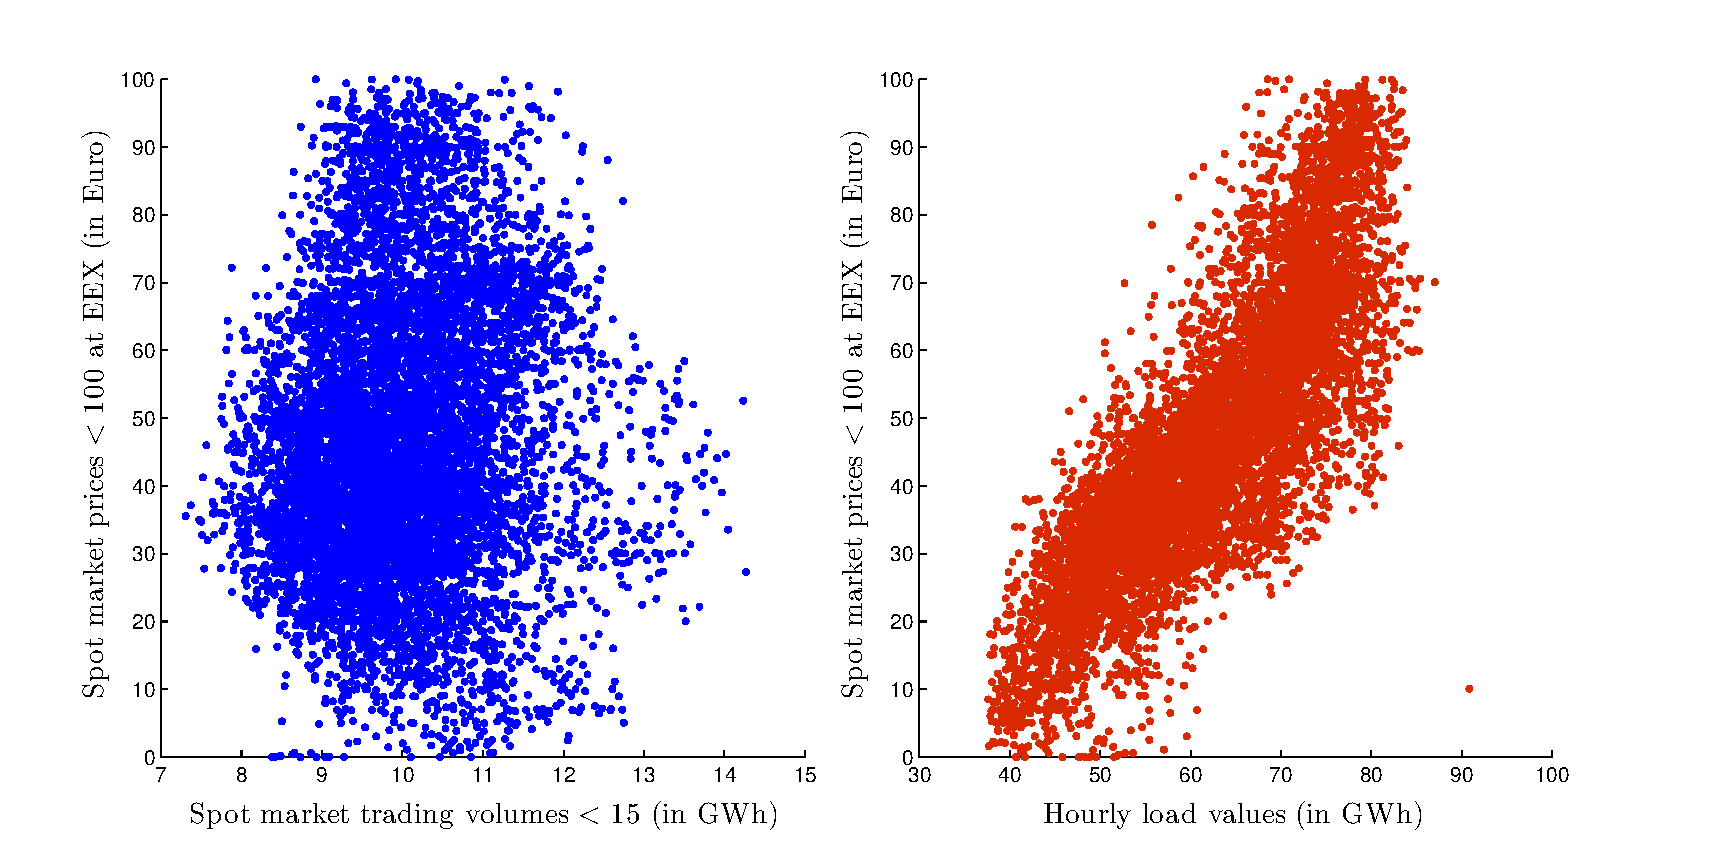
\includegraphics[width=1.0\textwidth, angle=0]{pricequant}
    \label{fig:load}            
\end{figure}
\end{frame}

\begin{frame}
  \frametitle{Market segments}

\begin{center}
\small
\begin{tabular}{rrrrr}
  \hline
Price & Average price  & Average quantity & Number of & Percentage of \\
intervals& (Euro/MWh) &  (MWh) &  prices & of total prices\\
  \hline\hline
$0\leq p<20$ & 12.67 & 46,111.63 & 611 & 6.98\% \\
$20\leq p<40$ & 31.35 & 54,103.50 & 3,003 & 34.28\% \\
$40\leq p<60$ & 49.00 & 64,806.04 & 2,626 & 29.98\% \\
$60\leq p<80$ & 68.46 & 72,385.56 & 1,588 & 18.13\% \\
$80\leq p<100$ & 88.40 & 75,991.21 & 665 & 7.59\% \\
$100\leq p<\infty$& 176.06 & 76,482.34 & 266 & 3.04\% \\
   \hline
\end{tabular}  
\normalsize
\end{center}

\end{frame}

\subsection{Marginal and investment costs}

\begin{frame}
  \frametitle{Marginal and investment costs}
\begin{center}
  \begin{tabular}{rrr}
\hline
           & Variable costs & Investment costs\\
           &  (Euro/MWh)    &  (Euro/GW) \\
\hline\hline
     Hydro &        7.6 &    3,500\\

   Nuclear &        9.5 &    1,841 \\

   Lignite &       10.6 &    1,074 \\

 Hard coal &       16.1 &     971 \\

 Gas (CCGT) &       33.5 &     460 \\

Oil & 44            &   n/a\\

Pump &         80 &       n/a\\
\hline
\end{tabular}
\end{center}
\end{frame}

\section{Results}

\subsection{Scenario generation}

\begin{frame}
  \frametitle{Scenario generation}
\begin{figure}[h]
  \centering
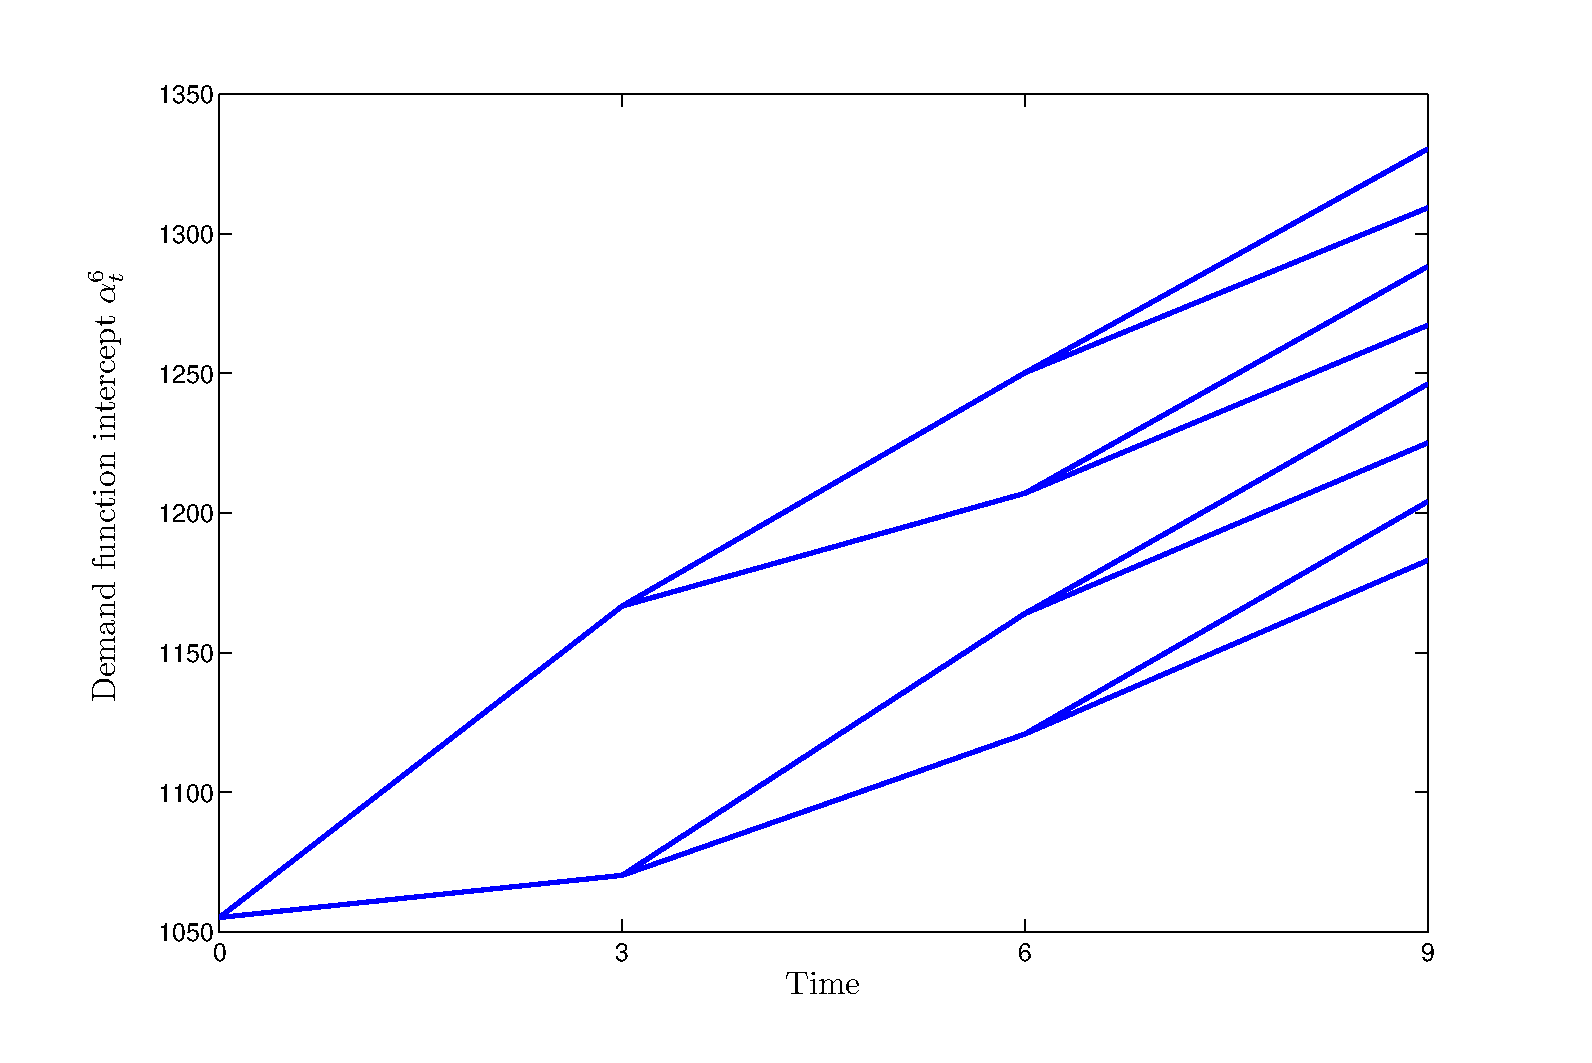
\includegraphics[width=1\textwidth]{intercept}
  \label{fig:intercept}
\end{figure}  
\end{frame}


\subsection{Solution of the MCP}

\begin{frame}
  \frametitle{Production in the initial node $q_{i,0}^{m}$ (in MWh)}
  \begin{center}
\scriptsize
      \begin{tabular}{rrrrrrr}
\hline
           &     $m=1$ &     $m=2$ &     $m=3$ &     $m=4$ &     $m=5$ &     $m=6$ \\
\hline\hline
       Rwe &    10,945.21  &    13,590.03  &    17,150.64  &    20,586.19  &    21,872.07  &    21,984.52  \\

       EON &    10,945.21  &    13,592.14  &    17,150.64  &    20,586.09  &    21,871.99  &    21,984.48  \\

    Vattenfall &    10,940.85  &    13,590.03  &    15,273.00  &    15,273.00  &    15,273.00  &    15,273.00  \\

      EnBW &    10,528.00  &    10,528.00  &    10,528.00  &    10,528.00  &    10,528.00  &    10,528.00  \\
\hline
\end{tabular}
\normalsize
  \end{center}
\end{frame}



\begin{frame}
  \frametitle{Sensitivity analysis}

  \begin{itemize}
  \item Investment quantities in the initial node $I_{i,0}$ (in MW) with $\rho=0.025$
  \end{itemize}

\begin{center}
  \begin{tabular}{rrrrr}
\hline
           &       $\nu=0.99$ &       $\nu=0.95$ &        $\nu=0.9$ &       $\nu=0.85$ \\
\hline\hline
 Vattenfall  &      5,015.93  &      4,832.23  &      4,626.18  &      4,516.54  \\

     EnBW  &      9,582.64  &      9,405.55  &      9,229.64  &      9,120.00  \\
\hline
\end{tabular}
\end{center}

\begin{itemize}
\item Investment quantities in the initial node $I_{i,0}$ (in MW) with $\nu=0.95$
\end{itemize}

\begin{center}
  \begin{tabular}{rrrrr}
\hline
           &      $\rho=0.025$ &       $\rho=0.03$ &      $\rho=0.035$ &       $\rho=0.04$ \\
\hline\hline
Vattenfall &      4,832.23  &      4,908.60  &      4,984.96  &      5,061.33  \\

      EnBW &      9,405.55  &      9,458.19  &      9,510.83  &      9,563.47  \\
\hline
\end{tabular}  
\end{center}

\end{frame}